\documentclass[a4paper,11pt]{article}

%% Language and font encodings
\usepackage[spanish,es-tabla]{babel}
\usepackage[utf8x]{inputenc}
%\usepackage{natbib}
\usepackage{booktabs}
\usepackage{tabu}
\usepackage[T1]{fontenc}
\usepackage{subcaption}
\usepackage{float}
\usepackage{amssymb}
\usepackage{multirow}
\usepackage{comment}
\usepackage{times} % pára el tipo de letra arial
\usepackage{wrapfig}
\usepackage{cite}
%% Sets page size and margins
\usepackage[a4paper,top=1.8cm,bottom=1.8cm,left=1.5cm,right=1.5cm,marginparwidth=1.75cm]{geometry}

%% Useful packages
\usepackage{amsmath}
\usepackage{graphicx}
%\usepackage{apacite}
\usepackage[colorinlistoftodos]{todonotes}
\usepackage[colorlinks=true, allcolors=blue]{hyperref}

\renewcommand{\labelenumii}{\theenumii}
\renewcommand{\theenumii}{\theenumi.\arabic{enumii}.}

\title{ 
	
	NeoArgos-tools: Un \textit{Pipeline} de Detección \textit{In-silico} de Neoantígenos de Cáncer para el Desarrollo de Vacunas Personalizadas
}

%\title{Desarrollo de una Aplicación Web para la Detección de Neoantígenos en el Marco de Desarrollo %de Vacunas Personalizadas para Tratar el Cáncer }
%\author{Vicente Machaca  e Yván Túpac}
\author{}
%\date{\today}
\date{}

\begin{document}
	

	
	
	
	
	
	
	
	%\maketitle

\part*{Propuesta de la Investigación}

\section{Título}
Desarrollo de una herramienta  para la detección \textit{in silico} de neoantígenos a partir de datos genómicos en el marco de desarrollo de vacunas personalizadas para tratar el cancer.

\section{Problema (5k) }

El cáncer representa el mayor problema de salud mundial \cite{siegel2023cancer}. Además, según el instituto de investigación del cáncer del Reino Unido, se ha registrado más de 18 millones de nuevos casos y 10 millones de muertes en el 2020 \cite{cancerUK2023}. Más alarmante aún, se predice que habrá 28 millones de nuevos casos por año alrededor del 2040, si la incidencia se mantiene estable y el crecimiento de la población y el envejecimiento continúan de acuerdo con las tendencias recientes \cite{cancerUK2023_2}. Esto representa un aumento del 54.9\% con respecto a 2020 y se espera que sea mayor en hombres (aumento del 60.6\%) que en mujeres (aumento del 48.8\%).	A todo esto, se sabe que los métodos tradicionales basados en cirugías, radioterapias y quimioterapias tienen baja efectividad y adversos efectos secundarios \cite{peng2019neoantigen}. En este contexto, surge el desarrollo de la inmunoterapia de cáncer, que tiene como objetivo estimular el sistema inmunológico de un paciente \cite{borden2022cancer}. Existen varios tratamientos como: vacunas personalizadas; terapias de células T adoptivas; e inhibidores de puntos de control inmunológico. De estos, las vacunas basadas en \textbf{neoantígenos} han demostrado un gran potencial, al potenciar las respuestas de las células T y es considerada la de mayor probabilidad de éxito \cite{borden2022cancer}. También, los neantígenos son utilizados en la terapia de bloqueo de puntos de control inmunológico. En este sentido, los neoantígenos son considerados biomarcadores predictivos y objetivos de tratamiento sinérgico en la inmunoterapia del cáncer \cite{fang2022neoantigens}.

A pesar de varios esfuerzos en el desarrollo de \textit{pipelines} y algoritmos, menos del 5\% de neoantígenos detectados activan el sistema immune \cite{de2020neoantigen, mill2022neoms, bulik2019deep, bassani2015mass, yadav2014predicting}. Según los autores de los \textit{pipelines} las razones son: 

\begin{enumerate}
	\item La no inclusión en conjunto de varias fuentes de información como DNA-seq, RNA-seq, y datos de \textit{Mass Spectrometry} (MS) \cite{kim2018neopepsee}. Por ejemplo, la mayoria de  propuestas no utiliza datos de MS; en la actualidad, existe una creciente información de estos datos y se estan aplicado a varios campos de la Bioinformática.
	
	\item  Uso herramientas de bajo desempeño para la predicción del enlace péptido-MHC (pMHC). La mayoria de aplicaciones, se basa en el uso de MHCFlurry \cite{o2020mhcflurry} y NetMHCpan4.1 \cite{reynisson2020netmhcpan}. Sin embargo, actualmente, se cuenta con herramientas de mejor desempeño como: MixMHCpred \cite{gfeller2023improved},  Anthem \cite{mei2021anthem}, Acme \cite{hu2019acme} y ESM-GAT \cite{hashemi2023improved}.
	
	\item Para la etapa 3.2 de la Figura \ref{fig:vaccines} del material complementario, los autores no consideran  la predicción del enlace pMHC al TCR (pMHC-TCR) , varios autores consideran incluir esta tarea en trabajos futuros  \cite{rubinsteyn2018computational}.
	
	\item Finalmente y quizas la mas importante es no utilizar información de eventos de \textit{alternative splicing}, variaciones estructurales en el ADN y las mutaciones de fusión de genes, está información esta fuertemente relacionada con varios tipos de cáncer \cite{wood2020neoepiscope}.
\end{enumerate}

\section{Estado del arte o antecedentes (10k)}
	

	
El desarrollo de vacunas personalizadas contra el cáncer es un proceso largo y depende de la correcta detección de neoantígenos (ver Figura \ref{fig:vaccines} del material complementario). Estos neoantígenos son péptidos que solo están presentes en las células cancerosas. De esta forma, el objetivo de un tratamiento basado en vacunas personalizadas, es entrenar a los linfocitos del paciente (células T) para reconocer los neoantígenos y activar el sistema inmunológico \cite{de2020neoantigen, peng2019neoantigen}. El proceso consiste en: 
	
	
	
	
	\begin{enumerate}
		\item ETAPA I: Obtener muestras de tejido canceroso y saludable, Luego se secuencia ambos tejidos para obtener el ADN y/o ARN. Algunas propuestas incluyen información inmunopeptidoma de \textit{Mass Spectrometry} (MS).
		\item ETAPA II: Aquí realiza alineamiento de secuencias, se desarrolla un \textit{llamado de variantes} para detectar las variantes y/o mutaciones; y se anotan dichas variantes (detección de posibles neoantígenos). Esta etapa cuenta con varias herramientas con buen desempeño.
		\item ETAPA III: En esta etapa \textit{in-silico} se priorizan neoantígenos. Esta etapa es crucial y ha tenido bastante investigación los últimos años debido a su complejidad y la baja efectividad de propuestas actuales. Aquí, se toman los neoantígenos candidatos (péptidos) de la etapa anterior y se predice su afinidad con el \textit{Major Histocompatibility Complex} (MHC), este problema se conoce como \textit{pMHC binding}. Luego, se  evalúa la afinidad del pMHC para enlazarse al T-cell Receptor (TCR). Al finalizar esta etapa, se obtienen los neoantígenos.
		\item ETAPA IV: En esta etapa \textit{in-vitro}, se induce en laboratorio  a las células T del paciente a reconocer los neoantígenos. Aquí, se desarrollan las vacunas. Generalmente, esta etapa es desarrollada por biotecnólogos y biólogos.
		\item ETAPA V: Finalmente, el médico oncólogo realiza la evaluación clínica de la vacuna.
	\end{enumerate}
	
	
	
	
	
	
	
	% AGREGAR LOS PIPELINES AGRUPADOS PAOR LA HERRAMITNAS QUE USAN, POR JEMPLO LA MAYORIA DE PIPELINES USAN XXX PARA ALINEAMIENT  Y  XXX PARA, LUEGO LU ...


\begin{figure}[h]	
		\centering
		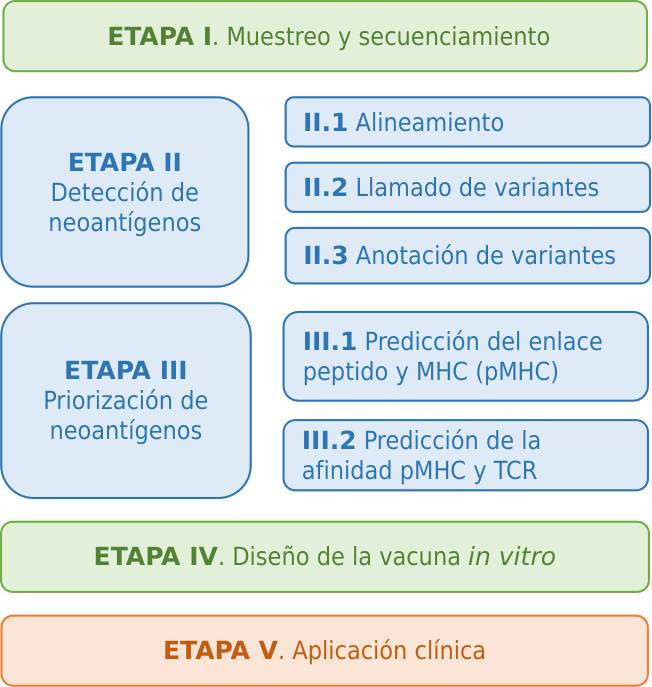
\includegraphics[width=0.4\textwidth]{../img/vaccines/pipeline2}	
	\caption{Marco de desarrollo para la elaboración de vacunas personalizadas contra el cáncer basadas en neoantígenos. Se detalla cada fase enfatizando el desarrollo \textit{in-silico}. Fuente: Elaboración propia.}
	\label{fig:vaccines}
\end{figure}
	
	
La detección \textit{in-silico} de neoantígenos se basa en la ETAPA II y III (ver Figura \ref{fig:vaccines} del material complementario). En este contexto, debido a la complejidad del proceso y la cantidad de métodos existentes, se han desarrollado software y \textit{pipelines} para facilitar el uso de estas herramientas. En la Tabla \ref{tab:review_pipelines} del material complementario, presentamos los \textit{pipelines} publicados a partir del 2018. Estos \textit{pipelines} utilizan diferentes tipos de información como entrada, así PGV Pipeline \cite{rubinsteyn2018computational} y PEPPRMINT \cite{zhou2023prioritizing} utilizan DNA-seq; sin embargo, otras herramientas como PGNneo \cite{tan2023pgnneo}, NAP-CNB \cite{wert2021predicting}, NaoANT-HILL \cite{coelho2020neoant}, ProGeo-neo \cite{li2020progeo}, ScanNeo \cite{wang2019scanneo} y Neopepse \cite{kim2018neopepsee} utilizan RNA-seq porque estas secuencias encapsulan mejor la información de mutaciones y \textit{non-coding regions} de ADN \cite{tan2023pgnneo}. 

Con el objetivo de reducir la complejidad de los \textit{pipelines}, otras propuestas han optado por utilizar Variant Calling Format (VCF), como entrada. Estos archivos, contienen información de las mutaciones y son obtenidas a partir de métodos de alineamiento y llamado de mutaciones (ETAPA II.1 y ETAPA II.3 de la Figura \ref{fig:vaccines} del material complementario). De esta forma, herramientas como Valid-Neo \cite{terai2022valid}, HLA3D \cite{li2022hla3d}, Neoepiscope \cite{wood2020neoepiscope} , pVACtools \cite{hundal2020pvactools} y NeoPredPipe \cite{schenck2019neopredpipe}, reducen la cantidad de herramientas utilizadas en la deteccion de neoantígenos; sin embargo, los resultados obtenidos, pueden ser inferiores comparado con herramientas que usan DNA-seq y RNA-seq. 

Adicionalmente, para una correcta detección de neoantígenos, es necesario contar con la secuenciación de proteínas Major Histocompatibility Complex (MHC) o Human Leukocyte Antigens (HLA). Es necesario contar con estas proteínas porque, son utilizadas para predecir la unión entre posibles neoantígenos al MHC (pMHC: ETAPA III.1 de la Figura \ref{fig:vaccines} del material complementario). Estas proteínas son codificadas por genes altamente polimórficos, esto proporciona una variación sustancial en la unión de péptidos (neoantígenos), influyendo de esta manera en el conjunto de péptidos presentados a las células T. \cite{abualrous2021major}. En este contexto,  los \textit{pipelines} Valid-NEO \cite{terai2022valid}  y NeoPredPipe \cite{schenck2019neopredpipe} y Neopepsee \cite{kim2018neopepsee} solicitan como entrada estas proteínas (HLA); mientras que las otras predicen esta información a partir de DNA-seq. Desde un punto de vista de usabilidad, obtener los tipos de HLA, implica un esfuerzo inncesario para el usuario.

%De esta la propuesta presenta una contribución en la disciplina de Bioinformática al plantear el uso de RNA-seq, DNA-seq en conjuno de datos Mass Spectrometry y además de que permiten predecir los tipos de proteínas HLA. Además, se va a incluir el uso de información de variaciones estructurales, fusión de genes y eventos de \textit{alternative splicing}. Estos fenómenos estan relacionados con varios tipos de cáncer \cite{wood2020neoepiscope} y aún no son utilizados por los pipelines estudiados en el estado del arte.  Finalmente, la propuesta presenta una contribución a la sub-area de Computación y Ciencias de la Información al incluir el desarrollo de un modelo \textit{Transformers} para la predicción del enlace pMHC y pMHC-TCR.  Este modelo aplicará fine-tuning de modelos BERT pre-entrenados en grandes bases de datos de proteínas. Según trabajos previos, los modelos Transformers obtienen mejores resultados que otras herramientas del estado del arte.
La presente propuesta ofrece una valiosa contribución a la disciplina de Bioinformática al proponer la integración de datos genómicos RNA-seq y DNA-seq, en combinación con datos de Mass Spectrometry.Además, también se va a incorporar información sobre variaciones estructurales, fusiones de genes y eventos de \textit{alternative splicing}, fenómenos que han sido vinculados a diversos tipos de cáncer \cite{wood2020neoepiscope} y que aún no son considerados por los pipelines examinados en el estado del arte. Adicionalmente, la propuesta presenta una contribución significativa en la sub-area de la Computación y Ciencias de la Información al introducir el desarrollo de un modelo basado en \textit{Transformers} para la predicción del enlace pMHC y pMHC-TCR. Este modelo empleará técnicas de fine-tuning utilizando modelos BERT pre-entrenados en extensas bases de datos de proteínas. Según investigaciones previas, los modelos Transformers han demostrado obtener resultados superiores en comparación con otras herramientas del estado del arte como NetMHCpan4.1 \cite{reynisson2020netmhcpan} y MHCflurry \cite{o2020mhcflurry}."


%En resumen, el desarrollo de \textit{pipelines} para la detección de neoantígenos es un campo de investigación significativo y de gran envergadura. Además, se está viendo favorecido por el crecimiento exponencial de la información genómica y los avances recientes en inteligencia artificial. 



% falta mencioan porque usan MS


	
\begin{table}[h]
	\caption{Lista de \textit{pipelines} desarrollados desde el 2018 hasta la actualidad para la detección de neoantígenos.GN: Expresión de genes, VA: anotación de variantes.}
	\label{tab:review_pipelines}
 \centering
	\setlength{\tabcolsep}{0.5em} % for the horizontal padding
	{\renewcommand{\arraystretch}{1.8}% for the vertical padding
    {\footnotesize
    \begin{tabular}{lllp{2cm}p{8.5cm}p{2cm}}
	\textbf{Nombre} & \textbf{Año}  & \textbf{Ref.}                                 & \textbf{Entrada}                                         & \textbf{Salida}    & \textbf{Herramientas}                                 \\ \hline
	
	PEPPRMINT         & 2023 &\cite{zhou2023prioritizing}         & DNA-seq                                                  & BWA, Mutect, Strelka, ANNOVAR, OptiType, PEPPRMINT, netMHCpan4.1 & Neoantígenos                                        \\

	PGNneo & 2023	& \cite{tan2023pgnneo}	& VCF, RNA-seq y MS data & Trimmomatic, BWA, SAMtools, GATK, Picard, OptiType, Annovar, Bedtools, MaxQuant, NetMHCpan4.1, Blastp	& Neoantígenos \\
	
	Valid-NEO       & 2022 &\cite{terai2022valid}             & VCF y HLA          & Neoantígenos  \\
	
	HLA3D & 2022	& \cite{li2022hla3d}	& VCF, HLA, SMG y HBV	& MHCcluster, SAVES, PROCHECK, CoDockPP, Verify 3D, ERRAT, ClusterW2, 3Dmol, PSRPRED4.0, MHCf lurry, CoDockPP & Neoantígenos \\
	
	
	
	NAP-CNB         & 2021 &\cite{wert2021predicting}         & RNA-seq                                                  & Star, Picard, GATK, SplitNCigarsReads, MuTect2, Cufinks, Epi-Seq, pVAC,seq, Neoantimon, MuPeXI, BLOSUM62 &  Neoantígenos                                       \\
	
	NeoANT-HILL     & 2020 &\cite{coelho2020neoant}           & RNA-seq y VCF                   & GATK, Mutect2, Optitype, NetMHC, NetMHCpan, NetMHCCcons, NetMHCstapan, PickPoket, SMM, SMMPMBEC, MHCflurry, NetMHCIIpan, NN-align, SMM-align, Sturniolo, Kallisto     & Neoantígenos,GE  \\
	
	Neoepiscope     & 2020 &\cite{wood2020neoepiscope}        & VCF y BAM            & BWA, Bowtie2, Pindel, MuSE, RADIA, SomaticSniper, VarScan2, GATK, HapCUT2       & Neoantígenos                          \\
	
	ProGeo-neo      & 2020 &\cite{li2020progeo}               & RNA-seq y VCF           & SRA Toolkit, BWA, GATK, Bcftools, ANNOVAR, Kallisto, OptiType, NetMHCpan4.0, Picard             & Neoantígenos                                       \\
	
	pVACtools       & 2020 &\cite{hundal2020pvactools}        & VCF                                         & CWL36, Cromwell37, ADNc38, BWA-MEM25, HaplotypeCaller28, MHCflurry14, MHCnuggets15, NetChop17, INTEGRATE-Neo19 & Neoantígenos                                       \\
	
	NeoPredPipe     & 2019 &\cite{schenck2019neopredpipe}     & VCF y HLA                & ANNOVAR, POLYSOLVER, netMHCpan, PeptideMatch            & Neoantígenos,VA              \\
	
	ScanNeo         & 2019 &\cite{wang2019scanneo}            & RNA-seq                                                  & HISAT2, BEDTools, BWA-MEM, pVAC-Seq, NetMHC, NetMHCpan & Neoantígenos                                       \\
	
		
	Neopepsee       & 2018 &\cite{kim2018neopepsee}           & RNA-seq, VCF, HLA  & NetCTLpan, Swiss-Prot & Neoantígenos,GE    \\ 
	
	PGV Pipeline    & 2018 &\cite{rubinsteyn2018computational}& DNA-seq                                                  & BWA-MEN, BQSR, MuTect, Strelka, STAR, seq2hla, Vaxrank, Isovar, MHCtools, Varcode, pyEnsembl & Neoantígenos                                       \\
	

\end{tabular}
}	
}
\end{table}






\section{Resultados o avances previos (4k)}


%La propuesta del proyecto es la continuación de una serie de proyectos y publicaciones. Primero se inicio con el PROYECTO 01: ``Principales estrategias y métodos basados en deep learning para la detección de neoantígenos en el marco del desarrollo de vacunas personalizadas en la inmunoterapia del cáncer'' financiado por la Universidad La Salle y la Universidad Católica San Pablo. Este proyecto generó como resultado dos publicaciones: ``Deep Learning and Transformers in MHC-Peptide Binding and Presentation Towards Personalized Vaccines in Cancer Immunology: A Brief Review'' \cite{machaca2023deep} y ``Neoantigen Detection Using Transformers and Transfer Learning in the Cancer Immunology Context'' \cite{arceda2023neoantigen}. 
La propuesta del proyecto representa la continuación de una serie de iniciativas y publicaciones. Se inició con el PROYECTO 01: "Principales estrategias y métodos basados en deep learning para la detección de neoantígenos en el marco del desarrollo de vacunas personalizadas en la inmunoterapia del cáncer", financiado por las Universidades La Salle y Católica San Pablo. Este proyecto resultó en dos publicaciones: "Deep Learning and Transformers in MHC-Peptide Binding and Presentation Towards Personalized Vaccines in Cancer Immunology: A Brief Review" \cite{machaca2023deep} y "Neoantigen Detection Using Transformers and Transfer Learning in the Cancer Immunology Context" \cite{arceda2023neoantigen}.

%Tambien, recientemente hemos culminado la ejecución del PROYECTO 02: ``Desarrollo de una Aplicación Web para la Detección de Neoantígenos en el Marco de Desarrollo de Vacunas Personalizadas para Tratar el Cáncer'', en este proyecto estamos desarrollando una aplicación para la detección de neoantígenos, enfocados en la predicción del enlace pMHC utilizando modelos Transformers y Transfer Learning. Asu vez, hemos sometido a revisión el paper ``Fine-tuning Transformers for Peptide-MHC Class I Binding Prediction''. Adicionalmente, esta propuesta de PROCIENCIA es el trabajo futuro de la tesis de doctorado en Ciencia de la Computación del investigador principal Vicente Machaca Arceda. La tesis titula: ``Detección \textit{in Silico} de Neoantígenos Utilizando Transformers y Transfer Learning en el Marco de Desarrollo de Vacunas Personalizadas para Tratar el Cáncer''. En la tesis se desarrolló los mismos objetivos del PROYECTO 02. Además, se logró la aceptación del artículo ``Transformers Meets Neoantigen Detection: A Systematic Literature Review'' al Journal of Integrative Bioinformatics (Q2).

Recientemente, hemos completado la ejecución del PROYECTO 02: "Desarrollo de una Aplicación Web para la Detección de Neoantígenos en el Marco de Desarrollo de Vacunas Personalizadas para Tratar el Cáncer". En este proyecto, hemos creado una aplicación centrada en la detección de neoantígenos, con un enfoque en la predicción del enlace pMHC mediante el uso de modelos Transformers y Transfer Learning. Además, hemos enviado para revisión el artículo "Fine-tuning Transformers for Peptide-MHC Class I Binding Prediction". Además, esta propuesta de PROCIENCIA también representa el trabajo futuro de la tesis de doctorado en Ciencia de la Computación del investigador principal, Vicente Machaca Arceda, titulada: "Detección \textit{in Silico} de Neoantígenos Utilizando Transformers y Transfer Learning en el Marco de Desarrollo de Vacunas Personalizadas para Tratar el Cáncer". La tesis aborda los mismos objetivos que el PROYECTO 02 y ha logrado la aceptación del artículo "Transformers Meets Neoantigen Detection: A Systematic Literature Review" en el Journal of Integrative Bioinformatics (Q2).

%Finalmente, esta en ejecución el PROYECTO 03 ``NeoArgos-tools: Un Pipeline de Detección In-silico de Neoantígenos de Cáncer para el Desarrollo de Vacunas Personalizadas''. Este proyecto finaliza en Junio de este año y tambien es financiado por la Universidad La Salle y a UCSP. Este representa el desarrollo de la primera versión de NeoArgos-tools (esta postulación a PROCIENCIA representa la versión 2). En esta primera versión, tomamos como entrada archivos Variant Calling File (VCF) y hemos mejorado el modulo de predicción del enlace pMHC en base a investigaciones previas de proyectos anteriores. 
Actualmente, estamos llevando a cabo el PROYECTO 03 "NeoArgos-tools: Un Pipeline de Detección In-silico de Neoantígenos de Cáncer para el Desarrollo de Vacunas Personalizadas", con fecha de finalización en junio de este año y financiamiento de las Universidades La Salle y UCSP. Este proyecto implica el desarrollo de la versión inicial de NeoArgos-tools (la postulación a PROCIENCIA corresponde a la versión 2). En la primera versión, utilizamos archivos Variant Calling File (VCF) como entrada y mejoramos el módulo de predicción del enlace pMHC según investigaciones previas de proyectos anteriores.

%Es importante menconar que en esta versión 2 de NeoArgos-tools, las mejoras planteadas son: utilizar datos genómicos como entrada al pipeline (RNS-seq y DNA-seq), además vamos a utilizar Mass Spectrometry (MS) para afinar la detección de neoantígenos. Luego, tambien vamos a incluir información de variantes estructurales y fusión de genes. Finalmente, vamos a desarrollar una interfaz gráfica.
Es relevante destacar que en la versión 2 de NeoArgos-tools, las mejoras propuestas incluyen el uso de datos genómicos como entrada al pipeline (RNS-seq y DNA-seq), la incorporación de Mass Spectrometry (MS) para refinar la detección de neoantígenos, la inclusión de información sobre variantes estructurales y fusión de genes, y el desarrollo de una interfaz gráfica.





\section{Justificación (4k)}

%El cáncer es el mayor problema de salud mundial; sin embargo, los métodos tradicionales basados en cirugías, radioterapias y quimioterapias tienen baja efectividad \cite{peng2019neoantigen}. En este contexto, los neoantígenos son factores clave en el desarrollo de vacunas contra el Cáncer  \cite{borden2022cancer,chen2021challenges,gopanenko2020main}. Si se logra desarrollar un método con un buen desempeño, la inmunoterapia del cáncer basada en el desarrollo de vacunas personalizadas, podría utilizarse como alternativa a otros métodos como radioterapias y quimioterapias. 

%El proyecto tiene dos contribuciones: CONTRIBUCIÓN 01: En el área de ciencia de la computación se va a desarrollar un modelo basado en \textit{Transformers} y Transfer Learning para la predicción del enlace pMHC, actualmente se tienen resultados previos que superan a otros del estado del arte. CONTRIBUCIÓN 02: En el área de la Bioinformática: el desarrollo del \textit{pipeline}, representa un reto resolviendo problemas de integración, alto costo computacional, heterogeneidad y modularidad. Además,  el \textit{pipeline} utilizará datos de \textit{Mass Spectrometry} (MS) y fusión de genes para obtener mejores resultados que otros métodos del estado del arte.

%Finalmente, con la culminación de este este proyecto, vamos a proceder con la segunda parte que involucra un trabajo interdisciplinario para el desarrollo \textit{in vitro} de las vacunas de neoantígenos. En una tercera etapa, se plantearán pruebas clínicas.
El cáncer constituye el principal desafío de salud a nivel global; no obstante, las técnicas convencionales basadas en cirugías, radioterapias y quimioterapias presentan una eficacia limitada \cite{peng2019neoantigen}. En este escenario, los neoantígenos emergen como elementos cruciales en la concepción de vacunas contra el cáncer \cite{borden2022cancer,chen2021challenges,gopanenko2020main}. Si se logra desarrollar un enfoque altamente efectivo, la inmunoterapia del cáncer, fundamentada en la creación de vacunas personalizadas, podría posicionarse como una alternativa a procedimientos más tradicionales, como radioterapias y quimioterapias.

En el proyecto se propone realizar dos contribuciones significativas: CONTRIBUCIÓN 01: En el ámbito de la ciencia de la computación, se llevará a cabo el desarrollo de un modelo basado en \textit{Transformers} y Transfer Learning para la predicción del enlace pMHC, con resultados previos que demuestran superar a otras propuestas en el estado del arte. CONTRIBUCIÓN 02: En el ámbito de la Bioinformática, la implementación del \textit{pipeline} plantea un desafío al abordar problemas de integración, alto costo computacional, heterogeneidad y modularidad. Además, este \textit{pipeline} incorporará datos de \textit{Mass Spectrometry} (MS), variaciones estructurales y fusión de genes con el objetivo de obtener resultados más sobresalientes que otros métodos presentes en el estado del arte.

Con la conclusión de este proyecto, se abrirá paso a la segunda fase, que implica una colaboración interdisciplinaria para llevar a cabo el desarrollo \textit{in vitro} de las vacunas de neoantígenos. En una tercera etapa, se contemplarán pruebas clínicas, marcando así un avance integral en la búsqueda de soluciones efectivas en la lucha contra el cáncer.







\section{Porqué es una investigación básica (3k)}
	
\section{Pregunta de investigación}	

¿El desarrollo de una herramienta in silico para la detección de neonatígenos a partir de datos genómicos es capaz de detectar correctmente geoantígenos de cancer?
	
\section{Objetivos de la investigación}
	
	\subsection{Objetivo general}
	
	Desarrollar una herramienta  para la detección \textit{in silico} de neoantígenos de cáncer a partir de datos genómicos.
	
	\subsection{Objetivos específicos}
	\begin{enumerate}
		\item \textbf{OBJ 1:} Evaluar alternativas para la integración de datos Mass Spectrometry (MS) con datos genómicos como RNA-seq y DNA-seq. 
		
		\item \textbf{OBJ 2:} Evaluar las herramientas STAR \cite{dobin2013star}, BWA \cite{li2009fast}, Bowtie2 \cite{langmead2019scaling} y Samtools \cite{danecek2021twelve} para determinar su aplicación en el alineamiento de secuencias.
		
		\item \textbf{OBJ 3:}
		Evaluar las herramientas GATK \cite{auwera2017somatic} y BFCtools \cite{danecek2021twelve} y determinar el uso apropiado de estas en el llamado de variantes. 
		
	
		
		\item \textbf{OBJ 4:} Analizar el uso de información de variaciones estructurales del ADN y mutaciones de fusión de genes. Se evaluará el desempeño de \textit{Arriba} \cite{uhrig2021accurate} y FusionQ \cite{liu2013fusionq}.


			\item \textbf{OBJ 5:} Evaluar la herramienta Isovar \cite{isovar2023} y Annovar \cite{wang2010annovar} para la anotación de variantes y la herramienta OptiType \cite{szolek2014optitype} para la predicción de tipos de HLA.
        %\item Evaluar métodos de detección de eventos de \textit{alternative splicing} y analizar la aplicación de estos al integrarse a la herramienta para la detección de neoantígenos.
		 
		\item \textbf{OBJ 6:} Implementar un modelo basado en \textit{transformers} para la predicción del enlace pMHC, esto como alternativa a NetMHCpan4.1 \cite{reynisson2020netmhcpan} o MHCflurry \cite{o2020mhcflurry}. Ya se cuenta con resultados previos de una propuesta que es superior a otras del estado del arte \cite{arceda2023neoantigen}.

        \item \textbf{OBJ 7:} Evaluar el modelo basado en \textit{transformers} para la predicción del enlace pMHC en otra tarea similar: la predicción  del enlace pMHC al TCR (pMHC-TCR). 
        
        \item \textbf{OBJ 8:} Implementar una interfaz gráfica que sirva como panel de administración para configurar y escoger las herramientas en cada fase del \textit{pipeline}.
		
        \item \textbf{OBJ 9:} Comparar el desempeño de la herramienta propuesta con otras herramientas del estado del arte.

		
	\end{enumerate}







\section{Metodología (5k)} 

Hemos dividido la propuesta en dos módulos: NeoArgosMut y NeoArgosAntigen. NeoArgosMut, se enfoca en el llamado y anotación de variantes, obteniéndose como salida neoantígenos candidatos. Luego, NeoArgosAntigen, prioriza estos antígenos, al predecir su afinidad al MHC (pMHC) y luego la afinidad del pMHC al TCR (pMHC-TCR). En la Figura \ref{fig:pipeline} del material complementario, mostramos estos módulos. 



\begin{figure}[h]	
		\centering
		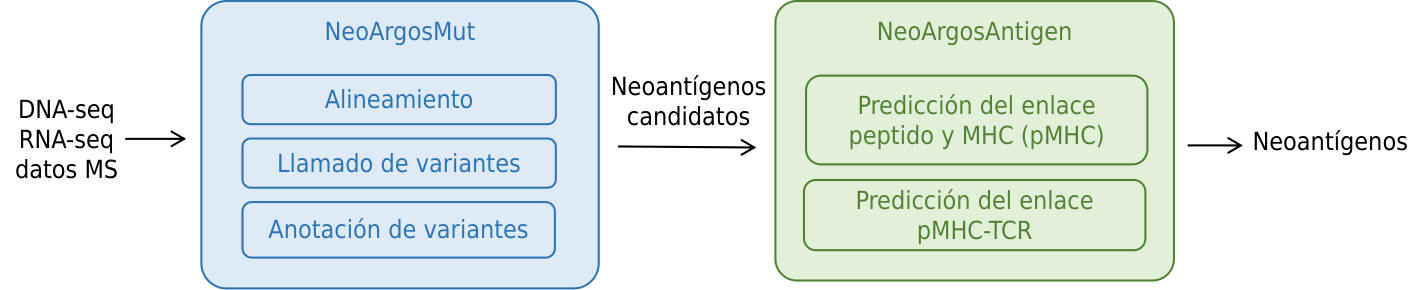
\includegraphics[width=\textwidth]{../img/pipeline/proposal_pipeline}	
	\caption{Representación de NeoArgosMut y NeoArgosAntigen para la detección de neoantígenos}
	\label{fig:pipeline}
\end{figure}


\subsection{NeoArgosMut}

Los objetivos específicos OBJ 1, OBJ  2, OBJ 3, OBJ 4 y OBJ 5 serán desarrollados con este modulo. Así, para el objetivo específico OBJ 1, NeoArgosMut, se encargará de recibir como entrada datos de DNA-seq, RNA-seq y Mass Spectrometry (MS). Se plantea utilzar la herramienta MaxQuant \cite{prianichnikov2020maxquant} para identificar las mutaciones a nivel de péptidos con ayuda de información de Mass Spectrometry (MS), esto  forma parte de la contribución del trabajo al incluir fuentes adicionales de información como MS.


Referente al objetivo específico OBJ 2, se plantea alinear las secuencias con uso de las herramientas BWA \cite{li2009fast}, Bowtie2 \cite{langmead2019scaling} y Samtools \cite{danecek2021twelve}. Adicionalmente, se planteará utilizar STAR, porque alinea mejor muestras tumorales \cite{rubinsteyn2018computational}. En esta etapa, se analizará y se determinará la mejor configuración y uso de cada herramienta. Como salida a esta etapa, se optiene archivos de alineamiento BAM.



Para el objetivo específico OBJ 3 que corresponde al llamado de variantes se utilizará MuTect y Strelka. Se plantea usar la unión de la información de ambos métodos tal como lo hizo \cite{zhou2023prioritizing} y \cite{rubinsteyn2018computational}. Como salida, se obtienen archivos VCF. Adicionalmente a otros \textit{pipelines}, en esta etapa tambien abordaremos el objetivo especifico OBJ 4 y utilizaremos información sobre la fusión de genes que se obtendrán de las herramientas \textit{Arriba} \cite{uhrig2021accurate} y FusionQ \cite{liu2013fusionq}. Esta forma parte de la contribución de este trabajo, porque se sabe que la mayoría de \textit{pipelines} tienen un bajo desempeño debido ausencia de información en su procesos de variantes estructurales y fusión de genes \cite{wood2020neoepiscope}. 



Finalmente el objetivo específico OBJ 5, se enfoca en la anotación ed variantes y predicción del tipo de HLA. En esta etapa se toman los archivos en formato VCF y se obtienen los péptidos generados a partir de estas variaciones o mutaciones. Estos péptidos representan los posibles neoantígenos. Para está tarea se va a utilizar Isovar \cite{isovar2023} y ANNOVAR \cite{wang2010annovar}, se evaluará su desempeño y se determinará cual de ellas usar bajo varios contextos. Luego, para obtener el tipo de HLA del paciente se va a utilizar la herramienta OptiType \cite{szolek2014optitype}. Otros \textit{pipelines} optan por solicitar al usuario la información del tipo de HLA; sin embargo, obtener el HLA a partir de las mismas secuencias de ADN, mejora considerablemente el desempeño general del pipeline y la accesibilidad del usuario. Al  finalizar esta etapa, se va a obtener los neoantígenos candidatos y los tipos de HLA.


\subsection{NeoArgosAntigen}

Los objetivos específicos OBJ 6, OBJ  7, OBJ 8, y OBJ 9 serán desarrollados con este modulo. NeoArgosAntigen, toma como entrada los neoantígenos candidatos y los tipos de HLA generados por NeoArgosMut. Esta prioriza estos neoantígenos. Esta priorización la realiza en base a la predicción del enlace de los neoantígenos al MHC, tambien conocido como predicción del enlace pMHC. Posteriormente se plantea predecir la afinidad del pMHC al TCR. El módulo se divide en dos partes: la predicción del enlace pMHC y la afinidad del pMHC al TCR. Ambas toman como entrada dos secuencias de proteínas, luego se necesita predecir su afinidad (regresión) o el enlace (clasificación). En resumen, las proteínas se pueden representar como $p = \{ A, ... , Q \}$ y $q = \{ A, N, ... ,Q, E, G \}$. Luego, tenemos que  predecir la probabilidad del enlace o afinidad entre $p$ y $q$. 


\begin{figure}[H]
	\centering
	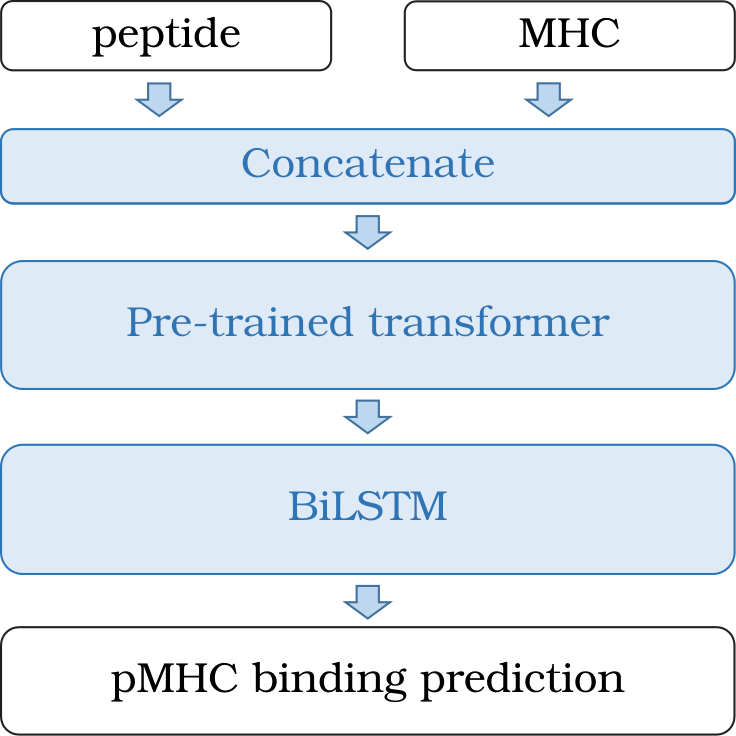
\includegraphics[width=0.30\textwidth]{../img/pipeline/proposal_pmhc}
	\caption{Modelo  \textit{transformer} seguido de BiLSTM para predecir el enlace pMHC.}
	\label{fig:proposal}
\end{figure}



Referente al objetivo específico OBJ 6, sobre el problema de predicción del enlace pMHC, se va a utilizar modelos BERT pre-entrenados y se realizará \textit{fine-tuning} agregando un bloque de capas BiLSTM, y otra basada en grafos. Luego se volverá a entrenar estos modelos con una base de datos compuesta por muestras de \cite{zhang2022hlab} y \cite{gfeller2023improved}. Se propone la arquitectura de la Figura \ref{fig:proposal} del material complementario. Como se puede ver, la entrada son dos secuencias de proteínas: el péptido y el MHC. Luego, el modelo basado en transformers está compuesto por un modelo pre-entrenado y un bloque de capas BiLSTM, esta propuesta se basó en el trabajo de \cite{zhang2022hlab}. En esta etapa también. se va a evaluar el desempeño de varios modelos BERT pre-entrenados como: TAPE \cite{rao2019evaluating}, ProtBERT-BFD \cite{elnaggar2021prottrans} y ESM2 \cite{lin2023evolutionary} cada una con 92 millones, 420 millones, 650 millones parámetros respectivamente. Adicionalmente, TAPE fue entrenado con 30 millones de proteínas, ProtBERT-BFD con 2122 millones de proteínas y 60 millones de proteínas para ESM-2. En base a trabajos anteriores propios, sabemos que el uso de TAPE y el modelo más pequeño de ESM2 tienen buenos resultados \cite{arceda2023neoantigen}. Además, por investigaciones previas propias sabemos que podemos superar el desempeño de las mejores herramientas del estado del arte como NetMHCpan4.1 \cite{reynisson2020netmhcpan} y MHCflurry \cite{o2020mhcflurry}.



Para el objetivo específico OBJ 7 para la predicción del enlace pMHC y TCR (pMHC-TCR), se utilizará la misma metodologúa del objetivo 6, según recomendaciones de otros autores \cite{li2020progeo, myronov2023bertrand}. Sin embargo, se va reentrenar el modelo para adaptarse a este nuevo problema, se utilizarán muestras de \cite{li2020progeo} y la base de datos de VDJdb \cite{shugay2018vdjdb}. Al finalizar esta etapa, se obtendrán los neonatígenos priorizados.


Luego, para lograr el objetivo especifico OBJ 8 referente al desarrollo de una interfaz gráfica para la configuración y selección de herramientas se va a desarrollar una herramienta similar a Orange Machine Learning. Por ejemplo, en la Figura \ref{fig:gui} del material complementario se muestra el prototipo de la interfaz gráfica. En el panel izquierdo se muestran las posibles herramientas, de las cuales el usario podrá escoger y configurar. En color azul, se resaltan las herramientas que representan una conribución en este trabajo. Luego, en el panel derecho, se muestra como el usuario puede realizar el flujo de actividades con las herramientas que ha seleccionado.

Finalmente, para lograr desarrollar el objetivo especifico OBJ 9, se va a comparar el resultado de la propuesta con otros pipelines del estado del arte. En la Tabla \ref{tab:review_pipelines} del material complementario se detallan estas herramientas. La comparación se realizará con las herramientas PEPPRMINT, HLA3d, ProGeoNeo y pVACtools. 



\begin{figure}[H]
	\centering
	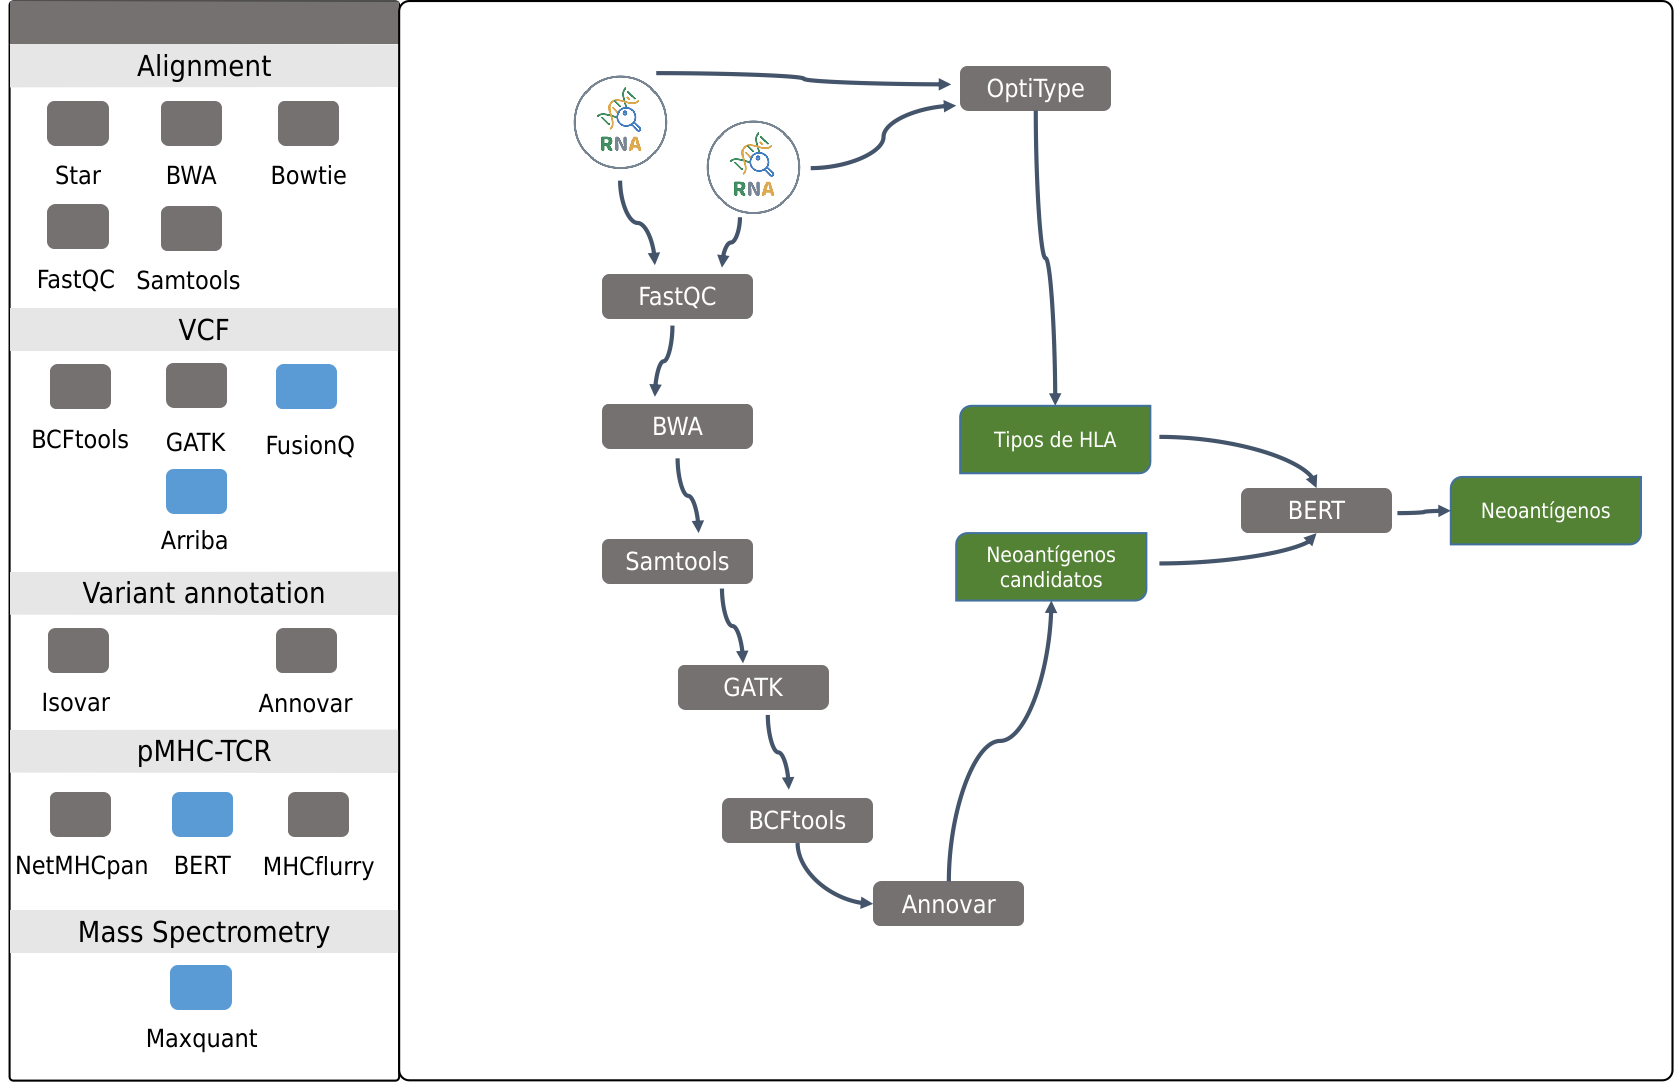
\includegraphics[width=\textwidth]{../img/proposal/gui2}
	\caption{Prototipo de la interfz gráfica de la herramienta para la detección ed neoantígenos. En el panel izquierdo se muestran las posibles herramientas, de las cuales el usario podrá escoger y configurar. En color azul, se resaltan las herramientas que representan una conribución en este trabajo. Luego, en el panel derecho, se muestra como el usuario puede realizar el flujo de actividades con las herramientas que ha seleccionado.}
	\label{fig:gui}
\end{figure}


\section{Limitaciones (5K)}

lIMITACIONES Y ESTRATEGIAS ABORADADAS


\section{Resumen (5K)}


\section{Describa el equipamiento e infraestructura disponible (5k)}

\section{Resultados esperados}

\section{Cronograma de Actividades}

\section{Sostenibilidad de la propuesta (5k)}

\section{Impacto Científico de la propuesta (5k)}






%\bibliographystyle{apalike}
\bibliographystyle{IEEEtran}
\bibliography{../bibliography_thesis}

	
\end{document}